\documentclass[12pt]{article}

\title{Initial conditions for SIR}
\author{Jan Medlock et al.}

\usepackage{microtype}
\usepackage{tikz}
\usepackage{hyperref}
\hypersetup{breaklinks}
\hypersetup{pdfborder=0 0 0}
\usepackage{amsmath}
\DeclareMathOperator{\Prob}{Prob}
\newcommand{\md}{\mathrm{d}}
\renewcommand{\vec}[1]{\mathbf{#1}}
\newcommand{\mat}[1]{\mathbf{#1}}


\begin{document}

\maketitle

\section{Model}

\begin{subequations}
  \begin{align}
    P_{\mathrm{S}}(a)
    &= \Prob\{\text{in compartment $\mathrm{S}$ at age $a$}\},\\
    p_{\mathrm{I}}(a, r)
    &= \Prob\{\text{in compartment $\mathrm{I}$ at age $a$ and
      duration $r$}\},\\
    P_{\mathrm{R}}(a)
    &= \Prob\{\text{in compartment $\mathrm{R}$ at age $a$}\},
  \end{align}
\end{subequations}
for $a \geq 0$ and $0 \leq r \leq a$.

\begin{figure}
  \begin{center}
    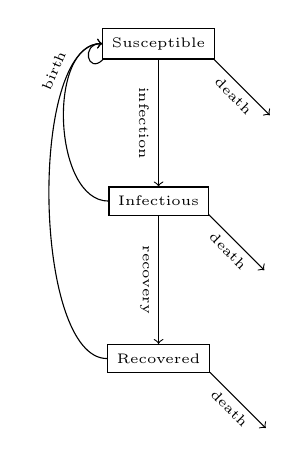
\begin{tikzpicture}[compartment/.style = {rectangle, draw}, font=\fontsize{5pt}{6}\selectfont]
  % Compartments.
  \node at (0, 9) [compartment, name=Susceptible] {Susceptible};
  \node at (0, 7) [compartment, name=Infectious] {Infectious};
  \node at (0, 5) [compartment, name=Recovered] {Recovered};

  \draw [->] (Susceptible)
             to node [rotate=-90, below] {infection}
             (Infectious);
  \draw [->] (Infectious)
             to node [rotate=-90, below] {recovery}
             (Recovered);

  % Births
  \draw [->] (Susceptible.196)
             to [out=225, in=180, looseness=3.5] node [] {}
             (Susceptible.180);
  \draw [->] (Infectious.180)
             to [out=180, in=180, looseness=0.9] node [sloped, above, pos=0.85] {}
             (Susceptible.180);
  \draw [->] (Recovered.180)
             to [out=180, in=180, looseness=0.6] node [sloped, above, pos=0.8] {birth}
             (Susceptible.180);

  % Deaths
  \draw [->] (Susceptible.344)
             to node [sloped, below, yshift=1pt] {death}
             +(315: 1);
  \draw [->] (Infectious.345)
             to node [sloped, below, yshift=1pt] {death}
             +(315: 1);
  \draw [->] (Recovered.345)
             to node [sloped, below, yshift=1pt] {death}
             +(315: 1);
\end{tikzpicture}

  \end{center}
  \caption{Model diagram.}
  \label{model_diagram}
\end{figure}

For $a > 0$ and $0 < r \leq a$, the equilibrium probability densities
satisfy
\begin{subequations}
  \begin{align}
    P_{\mathrm{S}}(0)
    &= 1,
    \\
    \frac{\md P_{\mathrm{S}}}{\md a}
    &= - \left[h_{\text{infection}} + h_{\text{death}}(a)\right]
      P_{\mathrm{S}}(a),
    \displaybreak[0]\\
    p_{\mathrm{I}}(0, 0)
    &= h_{\text{infection}} P_{\mathrm{S}}(0),
    \\
    p_{\mathrm{I}}(a, 0)
    &= h_{\text{infection}} P_{\mathrm{S}}(a),
    \\
    \left(\frac{\partial}{\partial a}
    + \frac{\partial}{\partial r}\right)
    p_{\mathrm{I}}
    &= - \left[h_{\text{recovery}}(r) + h_{\text{death}}(a)\right]
      p_{\mathrm{I}}(a, r),
    \displaybreak[0]\\
    P_{\mathrm{R}}(0) &= 0,
    \\
    \frac{\md P_{\mathrm{R}}}{\md a} &=
    \int_0^a h_{\text{recovery}}(r) p_{\mathrm{I}}(a, r) \md r
    - h_{\text{death}}(a) P_{\mathrm{R}}(a),
  \end{align}
\end{subequations}
with
\begin{equation}
  P_{\mathrm{I}}(a) = \int_0^a p_{\mathrm{I}}(a, r) \md r
\end{equation}
and
\begin{equation}
  P(a) = P_{\mathrm{S}}(a) + P_{\mathrm{I}}(a) + P_{\mathrm{R}}(a).
\end{equation}


\subsection{Analysis}

Integrating the PDEs along the characteristics $r = a - a_0$ gives
\begin{subequations}
  \begin{align}
    P_{\mathrm{S}}(0)
    &= 1,
    \\
    \frac{\md P_{\mathrm{S}}}{\md a}
    &= - \left[h_{\text{infection}}  + h_{\text{death}}(a)\right]
      P_{\mathrm{S}}(a),
    \displaybreak[0]\\
    p_{\mathrm{I}}(0, 0)
    &= h_{\text{infection}} P_{\mathrm{S}}(0),
    \\
    p_{\mathrm{I}}(a, 0)
    &= h_{\text{infection}} P_{\mathrm{S}}(a),
    \\
    p_{\mathrm{I}}(a, r)
    &= S_{\text{recovery}}(r)
      \frac{S_{\text{death}}(a)}{S_{\text{death}}(a - r)}
      p_{\mathrm{I}}(a - r, 0),
    \displaybreak[0]\\
    P_{\mathrm{R}}(0) &= 0,
    \\
    \frac{\md P_{\mathrm{R}}}{\md a} &=
    \int_0^a p_{\text{recovery}}(r)
    \frac{S_{\text{death}}(a)}{S_{\text{death}}(a - r)}
    p_{\mathrm{I}}(a - r, 0)
    \md r
    - h_{\text{death}}(a) P_{\mathrm{R}}(a).
  \end{align}
\end{subequations}

Using
\begin{equation}
  \label{eq:integral_over_r}
  P_{\mathrm{I}}(a)
  = \int_0^a
  S_{\text{recovery}}(a - a_0)
  \frac{S_{\text{death}}(a)}{S_{\text{death}}(a_0)}
  p_{\mathrm{I}}(a_0, 0)
  \md a_0,
\end{equation}
gives
\begin{equation}
  \label{eq:integral_derivative}
  \begin{split}
    \frac{\md P_{\mathrm{I}}}{\md a}
    &= h_{\text{infection}} P_{\mathrm{S}}(a)
    \\ & \quad {}
    - \int_0^a
    p_{\text{recovery}}(r)
    \frac{S_{\text{death}}(a)}{S_{\text{death}}(a - r)}
    p_{\mathrm{I}}(a - r, 0)
    \md r
    \\ & \quad {}
    - h_{\text{death}}(a) P_{\mathrm{I}}(a).
  \end{split}
\end{equation}
Then
\begin{subequations}
  \begin{align}
    \frac{\md P}{\md a}
    &= - h_{\text{death}}(a) P(a), \\
    P(0) &= 1,
  \end{align}
\end{subequations}
so that
\begin{equation}
  P(a) = S_{\text{death}}(a).
\end{equation}

The constant-time birth hazard
(i.e.~$c_{\mathrm{v}} = 0$)
\begin{equation}
  h_{\text{birth}}(a) =
  \begin{cases}
    0 & \text{if $a < 4$}, \\
    \mu & \text{if $a \geq 4$},
  \end{cases}
\end{equation}
with
\begin{equation}
  \mu =
  \left[
    \int_4^{+\infty} S_{\text{death}}(a) \md a
  \right]^{-1},
\end{equation}
gives
\begin{equation}
  \int_0^{+\infty} h_{\text{birth}}(a) P(a) \md a
  = \int_0^{+\infty} h_{\text{birth}}(a) S_{\text{death}}(a) \md a
  = 1
  = P(0),
\end{equation}
so that the population size is constant, i.e.~zero growth rate.


\section{Numerical method}

To compute the probability densities, we used the Crank--Nicolson
method on characteristics and the composite trapezoid rule for the
integrals.  Given the age step $\Delta a$,
for $i \in \{0, 1, 2, \ldots, I - 1\}$ and
$j \in \{0, 1, 2, \ldots, i\}$, let $a^i = i \Delta a$, $r^j = j
\Delta a$, $P_X^i \approx P_X(a^i)$, and
$p_{\mathrm{I}}^i \approx p_{\mathrm{I}}(a^i, 0)$.
For each $i \in \{1, 2, \ldots, I - 1\}$, using the
Crank--Nicolson method \textbf{TODO: Is this actually C--N?}
on characteristics gives
\begin{subequations}
  \label{eq:numerical_method}
  \begin{align}
    P_{\mathrm{S}}^0
    &= 1,
    \\
    \frac{P_{\mathrm{S}}^i - P_{\mathrm{S}}^{i - 1}}{\Delta a}
    &= - \frac{1}{2} \left[h_{\text{infection}}
      + h_{\text{death}}(a^i)\right]
    P_{\mathrm{S}}^i
    \\ & \quad {}
    - \frac{1}{2} \left[h_{\text{infection}}
      + h_{\text{death}}(a^{i - 1})\right]
    P_{\mathrm{S}}^{i - 1},
    \displaybreak[0]\\
    p_{\mathrm{I}}^0 &= 0,
    \\
    p_{\mathrm{I}}^i &=
    \frac{1}{2} h_{\text{infection}} P_{\mathrm{S}}^i
    + \frac{1}{2} h_{\text{infection}} P_{\mathrm{S}}^{i - 1},
    \displaybreak[0]\\
    P_{\mathrm{R}}^0 &= 0,
    \\
    \begin{split}
      \frac{P_{\mathrm{R}}^i - P_{\mathrm{R}}^{i - 1}}{\Delta a}
      &= \frac{1}{2} \sum_{j = 0}^i
      p_{\text{recovery}}(r^j)
      \frac{S_{\text{death}}(a^i)}{S_{\text{death}}(a^{i - j})}
      p_{\mathrm{I}}^{i - j}
      \Delta a
      \\ & \quad {}
      + \frac{1}{2} \sum_{j = 0}^{i - 1}
      p_{\text{recovery}}(r^j)
      \frac{S_{\text{death}}(a^{i - 1})}{S_{\text{death}}(a^{i - 1 - j})}
      p_{\mathrm{I}}^{i - 1 - j}
      \Delta a
      \\ & \quad {}
      - \frac{1}{2} h_{\text{death}}(a^i) P_{\mathrm{R}}^i
      - \frac{1}{2} h_{\text{death}}(a^{i - 1}) P_{\mathrm{R}}^{i - 1},
    \end{split}
  \end{align}
\end{subequations}
with
\begin{equation}
  \label{eq:sum_over_r}
  P_{\mathrm{I}}^i
  = \sum_{j = 0}^i
  S_{\text{recovery}}(r^j)
  \frac{S_{\text{death}}(a^i)}{S_{\text{death}}(a^{i - j})}
  p_{\mathrm{I}}^{i - j}
  \Delta a,
\end{equation}
and
\begin{equation}
  P^i =  P_{\mathrm{S}}^i + P_{\mathrm{I}}^i + P_{\mathrm{R}}^i.
\end{equation}


\subsection{Analysis}

The Crank--Nicholson approximation of the survival in terms of the
hazard is
\begin{equation}
  \begin{split}
    \frac{S_{\text{death}}(a^i) - S_{\text{death}}(a^{i - 1})}
    {\Delta a}
    &= - \frac{1}{2} h_{\text{death}}(a^i) S_{\text{death}}(a^i)
    \\ &\quad {}
    - \frac{1}{2} h_{\text{death}}(a^{i - 1}) S_{\text{death}}(a^{i - 1}),
  \end{split}
\end{equation}
so that
\begin{equation}
  S_{\text{death}}(a^i)
  = \prod_{j = 1}^i
  \frac{1 - h_{\text{death}}(a^{j - 1}) \Delta a / 2}
  {1 + h_{\text{death}}(a^j) \Delta a / 2}.
\end{equation}
This gives
\begin{equation}
  \begin{split}
    \frac{S_{\text{death}}(a^{i - 1}) - S_{\text{death}}(a^i)}
    {S_{\text{death}}(a^{i - 1}) \Delta a}
    &= \frac{h_{\text{death}}(a^i) + h_{\text{death}}(a^{i - 1})}
    {2 + h_{\text{death}}(a^i) \Delta a}.
  \end{split}
\end{equation}

\textbf{TODO: \eqref{eq:sum_difference} should look like
  \eqref{eq:integral_derivative}.}
%
The difference of the sum \eqref{eq:sum_over_r} is
\begin{align}
  \label{eq:sum_difference}
  \begin{split}
    \frac{P_{\mathrm{I}}^i - P_{\mathrm{I}}^{i - 1}}{\Delta a}
    &=
    \sum_{j = 0}^i S_{\text{recovery}}(r^j)
    \frac{S_{\text{death}}(a^i)}{S_{\text{death}}(a^{i - j})}
    p_{\mathrm{I}}^{i - j}
    \\ & \quad {}
    - \sum_{j = 0}^{i - 1} S_{\text{recovery}}(r^j)
    \frac{S_{\text{death}}(a^{i - 1})}{S_{\text{death}}(a^{i - 1 - j})}
    p_{\mathrm{I}}^{i - 1 - j}
  \end{split}
  \displaybreak[0]\\
  \begin{split}
    &= p_{\mathrm{I}}^i
    + \sum_{j = 1}^i S_{\text{recovery}}(r^j)
    \frac{S_{\text{death}}(a^i)}{S_{\text{death}}(a^{i - j})}
    p_{\mathrm{I}}^{i - j}
    \\ & \quad {}
    - \sum_{j = 1}^i S_{\text{recovery}}(r^{j - 1})
    \frac{S_{\text{death}}(a^{i - 1})}{S_{\text{death}}(a^{i - j})}
    p_{\mathrm{I}}^{i - j}
  \end{split}
  \displaybreak[0]\\
  \begin{split}
    &= p_{\mathrm{I}}^i
    - \sum_{j = 1}^i \left[
      S_{\text{recovery}}(r^{j - 1})
      - S_{\text{recovery}}(r^j)
    \right]
    \frac{S_{\text{death}}(a^i)}{S_{\text{death}}(a^{i - j})}
    p_{\mathrm{I}}^{i - j}
    \\ & \quad {}
    - \sum_{j = 1}^i S_{\text{recovery}}(r^{j - 1})
    \frac{S_{\text{death}}(a^{i - 1}) - S_{\text{death}}(a^i)}
    {S_{\text{death}}(a^{i - j})}
    p_{\mathrm{I}}^{i - j}
  \end{split}
  \displaybreak[0]\\
  \begin{split}
    &= p_{\mathrm{I}}^i
    - \sum_{j = 1}^i
    \frac{S_{\text{recovery}}(r^{j - 1}) - S_{\text{recovery}}(r^j)}
    {\Delta a}
    \frac{S_{\text{death}}(a^i)}{S_{\text{death}}(a^{i - j})}
    p_{\mathrm{I}}^{i - j} \Delta a
    \\ & \quad {}
    -
    \frac{S_{\text{death}}(a^{i - 1}) - S_{\text{death}}(a^i)}
    {S_{\text{death}}(a^{i - 1}) \Delta a}
    \sum_{j = 0}^{i - 1} S_{\text{recovery}}(r^j)
    \frac{S_{\text{death}}(a^{i - 1})}{S_{\text{death}}(a^{i - 1 - j})}
    p_{\mathrm{I}}^{i - 1 - j} \Delta a
  \end{split}
  \displaybreak[0]\\
  \begin{split}
    &= p_{\mathrm{I}}^i
    - \sum_{j = 0}^i p_{\text{recovery}}(r^j)
    \frac{S_{\text{death}}(a^i)}{S_{\text{death}}(a^{i - j})}
    p_{\mathrm{I}}^{i - j} \Delta a
    \\ & \quad {}
    + p_{\text{recovery}}(0) p_{\mathrm{I}}^i \Delta a
    - \frac{S_{\text{death}}(a^{i - 1}) - S_{\text{death}}(a^i)}
    {S_{\text{death}}(a^{i - 1}) \Delta a}
    P_{\mathrm{I}}^{i - 1}
  \end{split}
  \displaybreak[0]\\
  \begin{split}
    &= p_{\mathrm{I}}^i
    - \sum_{j = 0}^i p_{\text{recovery}}(r^j)
    \frac{S_{\text{death}}(a^i)}{S_{\text{death}}(a^{i - j})}
    p_{\mathrm{I}}^{i - j} \Delta a
    \\ & \quad {}
    - \frac{1}{2} \left[h_{\text{death}}(a^i) P_{\mathrm{I}}^i
      + h_{\text{death}}(a^{i - 1}) P_{\mathrm{I}}^{i - 1}\right]
    \\ & \quad {}
    + p_{\text{recovery}}(0) p_{\mathrm{I}}^i \Delta a
    - \frac{S_{\text{death}}(a^{i - 1}) - S_{\text{death}}(a^i)}
    {S_{\text{death}}(a^{i - 1}) \Delta a}
    P_{\mathrm{I}}^{i - 1}
    \\ & \quad {}
    + \frac{1}{2} \left[h_{\text{death}}(a^i) P_{\mathrm{I}}^i
      + h_{\text{death}}(a^{i - 1}) P_{\mathrm{I}}^{i - 1}\right]
  \end{split}
  \displaybreak[0]\\
  \begin{split}
    &= p_{\mathrm{I}}^i
    - \sum_{j = 0}^i p_{\text{recovery}}(r^j)
    \frac{S_{\text{death}}(a^i)}{S_{\text{death}}(a^{i - j})}
    p_{\mathrm{I}}^{i - j} \Delta a
    \\ & \quad {}
    - \frac{1}{2} \left[h_{\text{death}}(a^i) P_{\mathrm{I}}^i
      + h_{\text{death}}(a^{i - 1}) P_{\mathrm{I}}^{i - 1}\right]
    \\ & \quad {}
    + p_{\text{recovery}}(0) p_{\mathrm{I}}^i \Delta a
    - \frac{1}{2}
    \frac{h_{\text{death}}(a^i) + h_{\text{death}}(a^{i - 1})}
    {1 + h_{\text{death}}(a^i) \Delta a / 2}
    P_{\mathrm{I}}^{i - 1}
    \\ & \quad {}
    + \frac{1}{2} \left[h_{\text{death}}(a^i) P_{\mathrm{I}}^i
      + h_{\text{death}}(a^{i - 1}) P_{\mathrm{I}}^{i - 1}\right]
  \end{split}
  \displaybreak[0]\\
  \begin{split}
    &= p_{\mathrm{I}}^i
    - \sum_{j = 0}^i p_{\text{recovery}}(r^j)
    \frac{S_{\text{death}}(a^i)}{S_{\text{death}}(a^{i - j})}
    p_{\mathrm{I}}^{i - j} \Delta a
    \\ & \quad {}
    - \frac{1}{2} \left[h_{\text{death}}(a^i) P_{\mathrm{I}}^i
      + h_{\text{death}}(a^{i - 1}) P_{\mathrm{I}}^{i - 1}\right]
    \\ & \quad {}
    + p_{\text{recovery}}(0) p_{\mathrm{I}}^i \Delta a
    \\ & \quad {}
    + \frac{1}{2} h_{\text{death}}(a^i)
    \left[P_{\mathrm{I}}^i
      - \frac{1 - h_{\text{death}}(a^{i - 1}) \Delta a / 2}
      {1 + h_{\text{death}}(a^i) \Delta a / 2}
      P_{\mathrm{I}}^{i - 1}\right]
  \end{split}
  \displaybreak[0]\\
  \begin{split}
    &= p_{\mathrm{I}}^i
    - \sum_{j = 0}^i p_{\text{recovery}}(r^j)
    \frac{S_{\text{death}}(a^i)}{S_{\text{death}}(a^{i - j})}
    p_{\mathrm{I}}^{i - j} \Delta a
    \\ & \quad {}
    - \frac{1}{2} \left[h_{\text{death}}(a^i) P_{\mathrm{I}}^i
      + h_{\text{death}}(a^{i - 1}) P_{\mathrm{I}}^{i - 1}\right]
    \\ & \quad {}
    + p_{\text{recovery}}(0) p_{\mathrm{I}}^i \Delta a
    \\ & \quad {}
    + \frac{1}{2} h_{\text{death}}(a^i)
    \left[P_{\mathrm{I}}^i
      - \frac{S_{\text{death}}(a^i)}{S_{\text{death}}(a^{i - 1})}
      P_{\mathrm{I}}^{i - 1}\right],
  \end{split}
  \displaybreak[0]\\
  \begin{split}
    &= p_{\mathrm{I}}^i
    - \frac{1}{2} \sum_{j = 0}^i
    p_{\text{recovery}}(r^j)
    \frac{S_{\text{death}}(a^i)}{S_{\text{death}}(a^{i - j})}
    p_{\mathrm{I}}^{i - j}
    \Delta a
    \\ & \quad {}
    - \frac{1}{2} \sum_{j = 0}^{i - 1}
    p_{\text{recovery}}(r^j)
    \frac{S_{\text{death}}(a^{i - 1})}{S_{\text{death}}(a^{i - 1 - j})}
    p_{\mathrm{I}}^{i - 1 - j}
    \Delta a
    \\ & \quad {}
    - \frac{1}{2} \left[h_{\text{death}}(a^i) P_{\mathrm{I}}^i
      + h_{\text{death}}(a^{i - 1}) P_{\mathrm{I}}^{i - 1}\right]
    \\ & \quad {}
    + \left\{
      p_{\text{recovery}}(0)
      + \frac{1}{2} h_{\text{death}}(a^i)
      \left[1 + p_{\text{recovery}}(0) \Delta a \right]
    \right\} \Delta a p_{\mathrm{I}}^i
    \\ & \quad {}
    - \frac{1}{2}
    \left[1 + h_{\text{death}}(a^i) \Delta a\right]
    \sum_{j = 0}^i p_{\text{recovery}}(r^j)
    \frac{S_{\text{death}}(a^i)}{S_{\text{death}}(a^{i - j})}
    p_{\mathrm{I}}^{i - j} \Delta a
    \\ & \quad {}
    + \frac{1}{2} \sum_{j = 0}^{i - 1}
    p_{\text{recovery}}(r^j)
    \frac{S_{\text{death}}(a^{i - 1})}{S_{\text{death}}(a^{i - 1 - j})}
    p_{\mathrm{I}}^{i - 1 - j}
    \Delta a
  \end{split}
\end{align}
\textbf{TODO: Shit. The first 4 terms are correct but the rest are
  hideous. Should $P_{\mathrm{I}}^i$ be the average over sums at $i$
  and $i - 1$?}

Then
\begin{subequations}
  \begin{align}
    P^0 &= 1,
    \displaybreak[0]\\
    \begin{split}
      \frac{P^i - P^{i - 1}}{\Delta a}
      &= - \frac{1}{2} \left[
        h_{\text{death}}(a^i) P^i
        + h_{\text{death}}(a^{i - 1}) P^{i - 1}
      \right],
    \end{split}
  \end{align}
\end{subequations}
so that
\begin{equation}
  \label{eq:discrete_total}
  \begin{split}
    P^i
    &= \frac{
      1 - h_{\text{death}}(a^{i - 1}) \Delta a / 2
    }{
      1 + h_{\text{death}}(a^i) \Delta a / 2
    } P^{i - 1}
    \\
    &= \prod_{j = 1}^i \frac{
      1 - h_{\text{death}}(a^{j - 1}) \Delta a / 2
    }{
      1 + h_{\text{death}}(a^j) \Delta a / 2
    }
    \\
    &= S_{\text{death}}(a^i).
  \end{split}
\end{equation}
The the constant-time birth hazard
(i.e.~$c_{\mathrm{v}} = 0$)
\begin{equation}
  h_{\text{birth}}(a) =
  \begin{cases}
    0 & \text{if $a < 4$}, \\
    \mu & \text{if $a \geq 4$},
  \end{cases}
\end{equation}
with
\begin{equation}
  \mu =
  \left[
    \sum_{a^i \geq 4}
    S_{\text{death}}(a^i)
    \Delta a
  \right]^{-1},
\end{equation}
gives
\begin{equation}
  \sum_{i = 0}^{I - 1}
  h_{\text{birth}}(a^i) P^i
  \Delta a
  = \sum_{i = 0}^{I - 1}
  h_{\text{birth}}(a^i) S_{\text{death}}(a^i)
  \Delta a
  = 1 = P_0,
\end{equation}
so that the population size is constant, i.e.~zero growth rate.


\subsection{Implementation}

\textbf{TODO: This section has not been updated yet.}

Numerical scheme \eqref{eq:numerical_method} can be written as
\begin{subequations}
  \begin{align}
    P_{\mathrm{S}}^0
    &= 1,
    \\
    \begin{split}
      - \left\{
        1
        - \left[h_{\text{infection}} + h_{\text{death}}(a^{i - 1 / 2})\right]
        \frac{\Delta a}{2}
      \right\} P_{\mathrm{S}}^{i - 1}
      \\ {}
      + \left\{
        1
        + \left[h_{\text{infection}} + h_{\text{death}}(a^{i - 1 / 2})\right]
        \frac{\Delta a}{2}
      \right\} P_{\mathrm{S}}^i
      &= 0,
    \end{split}
    \displaybreak[0]\\
    - h_{\text{infection}} P_{\mathrm{S}}^0
    + p_{\mathrm{I}}^0 &= 0,
    \\
    - \frac{h_{\text{infection}}}{2} P_{\mathrm{S}}^{i - 1}
    - \frac{h_{\text{infection}}}{2} P_{\mathrm{S}}^i
    + p_{\mathrm{I}}^i
    &= 0,
    \displaybreak[0]\\
    P_{\mathrm{R}}^0 &= 0,
    \\
    \begin{split}
      - \sum_{j = 0}^i
      p_{\text{recovery}}(r^{i - j})
      \frac{S_{\text{death}}(a^i)}{S_{\text{death}}(a^j)}
      \Delta a^2
      p_{\mathrm{I}}^j
      \\ {}
      - \left[1 - h_{\text{death}}(a^{i - 1 / 2}) \frac{\Delta a}{2}\right]
      P_{\mathrm{R}}^{i - 1}
      \\ {}
      + \left[1 + h_{\text{death}}(a^{i - 1 / 2}) \frac{\Delta a}{2}\right]
      P_{\mathrm{R}}^i
      &= 0.
    \end{split}
  \end{align}
\end{subequations}

Define the vectors
\begin{equation}
  \vec{x}_X =
  \begin{cases}
    \begin{pmatrix}
      P_X^0\\
      P_X^1\\
      \vdots\\
      P_X^{I - 1}
    \end{pmatrix}
    &
    \text{for $X \in \left\{\mathrm{S}, \mathrm{R}\right\}$},
    \\[4em]
    \begin{pmatrix}
      p_X^0\\
      p_X^1\\
      \vdots\\
      p_X^{I - 1}
    \end{pmatrix}
    &
    \text{for $X \in \left\{\mathrm{I}\right\}$},
  \end{cases}
\end{equation}
and let $\vec{x}$ be the $\vec{x}_X$'s stacked into a single vector,
\begin{equation}
  \vec{x} =
  \begin{pmatrix}
    \vec{x}_{\mathrm{S}}\\
    \vec{x}_{\mathrm{I}}\\
    \vec{x}_{\mathrm{R}}
  \end{pmatrix}.
\end{equation}

Define the block diagonal matrix
\begin{align}
  \mat{D} &=
  \begin{bmatrix}
    \mat{D}_{\mathrm{S}} & \mat{0} & \mat{0}
    \\
    \mat{0} & \bar{\mat{D}}_{\mathrm{I}} & \mat{0}
    \\
    \mat{0} & \mat{0} & \mat{D}_{\mathrm{R}}
  \end{bmatrix},
\end{align}
with blocks
\begin{subequations}
  \begin{align}
    \mat{D}_X &=
    \begin{bmatrix}
      1 & 0 & 0 & \hdots & 0
      \\
      - (1 - d_X^1) & 1 + d_X^1 & 0 & \hdots & 0
      \\
      0 & - (1 - d_X^2) & 1 + d_X^2 & \ddots & \vdots
      \\
      \vdots & \ddots & \ddots & \ddots & 0
      \\
      0 & \hdots & 0 & - (1 - d_X^{I - 1}) & 1 + d_X^{I - 1}
    \end{bmatrix},
    \\
    \bar{\mat{D}}_X &=
    \begin{bmatrix}
      1 & 0 & \hdots & 0 \\
      0 & 1 & \ddots & \vdots \\
      \vdots & \ddots & \ddots & 0 \\
      0 & \hdots & 0 & 1
    \end{bmatrix},
  \end{align}
\end{subequations}
where
\begin{subequations}
  \begin{align}
    d_{\mathrm{S}}^i
    &= \frac{1}{2} \left[h_{\text{infection}}
      + h_{\text{death}}(a^{i - 1 / 2})\right]
      \Delta a,
    \\
    d_{\mathrm{R}}^i
    &= \frac{1}{2} h_{\text{death}}(a^{i - 1 / 2}) \Delta a,
  \end{align}
\end{subequations}
for $i \in \{1, 2, \ldots, I - 1\}$.

Define the influx matrix
\begin{equation}
  \mat{F} =
  \begin{bmatrix}
    \mat{0} & \mat{0} & \mat{0}
    \\
    \mat{F}_{\mathrm{IS}} & \mat{0} & \mat{0}
    \\
    \mat{0} & \bar{\mat{F}}_{\mathrm{RI}} & \mat{0}
  \end{bmatrix},
\end{equation}
with blocks
\begin{subequations}
  \begin{align}
    \mat{F}_{XY} &=
    \begin{bmatrix}
      f_{XY}^0 & 0 & 0 & \hdots & 0
      \\
      f_{XY}^1 & f_{XY}^1 & 0 & \hdots & 0
      \\
      0 & f_{XY}^2 & f_{XY}^2 & \ddots & \vdots
      \\
      \vdots & \ddots & \ddots & \ddots & 0
      \\
      0 & \hdots & 0 & f_{XY}^{I - 1} &
      f_{XY}^{I - 1}
    \end{bmatrix},
    \displaybreak[0]\\
    \bar{\mat{F}}_{XY} &=
    \begin{bmatrix}
      \bar{f}_{XY}^{0, 0} & 0 & \hdots & 0
      \\
      \bar{f}_{XY}^{1, 0} & \bar{f}_{XY}^{1, 1} & \ddots & \vdots
      \\
      \vdots &  & \ddots & 0
      \\
      \bar{f}_{XY}^{I - 1, 0} & \bar{f}_{XY}^{I - 1, 1} & \hdots &
      \bar{f}_{XY}^{I - 1, I - 1}
    \end{bmatrix},
  \end{align}
\end{subequations}
where
\begin{subequations}
  \begin{align}
    f_{\mathrm{IS}}^i &=
    \begin{cases}
      h_{\text{infection}}
      & \text{for $i \in \{0\}$},
      \\
      \frac{1}{2} h_{\text{infection}}
      & \text{for $i \in \{1, 2, \ldots, I - 1\}$},
    \end{cases}
    \displaybreak[0]\\
    \bar{f}_{\mathrm{RI}}^{i, j} &=
    \begin{cases}
      0 & \text{for $i \in \{0\}$ and $j \in \{0\}$},
      \\
      p_{\text{recovery}}(r^{i - j})
      \frac{S_{\text{death}}(a^i)}{S_{\text{death}}(a^j)}
      \Delta a^2 &
      \begin{aligned}
        \text{for $i \in \{1, 2, \ldots, I - 1\}$}&\\
        \text{and $j \in \{0, 1, 2, \ldots, i\}$}&.
      \end{aligned}
    \end{cases}
  \end{align}
\end{subequations}

Define the vector
\begin{equation}
  \vec{b} =
  \begin{pmatrix}
    \vec{b}_{\mathrm{S}} \\
    \vec{0} \\
    \vec{0}
  \end{pmatrix},
\end{equation}
with
\begin{equation}
  \vec{b}_{\mathrm{S}} =
  \begin{pmatrix}
    1 \\
    0 \\
    \vdots \\
    0
  \end{pmatrix}.
\end{equation}

Define the matrix
\begin{equation}
  \mat{A} =
  \mat{D} - \mat{F}.
\end{equation}
The numerical scheme is then finding the vector $\vec{x}$ that solves
\begin{equation}
  \mat{A} \vec{x} = \vec{b}.
\end{equation}

The diagonal entries of $\mat{A}$ are non-negative if
\begin{equation}
  h_{\text{birth}}(a^0) \Delta a \leq 1,
\end{equation}
and the off-diagonal entries of $\mat{A}$ are non-positive if
\begin{equation}
  d_X^i \leq 1.
\end{equation}
Under these conditions, the entries of $\vec{x}$ are non-negative.


\section{$p_\mathrm{I}$ PDE}

To compute the probability densities, we used the Crank--Nicolson
method on characteristics.  Given the age step $\Delta a$,
for $i \in \{0, 1, 2, \ldots, I - 1\}$ and
$j \in \{0, 1, 2, \ldots, i\}$, let $a^i = i \Delta a$, $r^j = j
\Delta a$, $P_X^i \approx P_X(a^i)$, and
$p_{\mathrm{I}}^{i, j} \approx p_{\mathrm{I}}(a^i, r^j)$.
For each $i \in \{1, 2, \ldots, I - 1\}$
and $j \in \{1, 2, \ldots, i\}$,
using the Crank--Nicolson method on characteristics gives
\begin{subequations}
  \label{eq:pde_numerical_method}
  \begin{align}
    P_{\mathrm{S}}^0
    &= 1,
    \\
    \begin{split}
      \frac{P_{\mathrm{S}}^i - P_{\mathrm{S}}^{i - 1}}{\Delta a}
      &= - \frac{1}{2} \left\{
        \left[h_{\text{infection}}
          + h_{\text{death}}(a^i)\right]
        P_{\mathrm{S}}^i
      \right.
      \\ &
      \left. \quad\quad\quad {}
        + \left[h_{\text{infection}}
          + h_{\text{death}}(a^{i - 1})\right]
        P_{\mathrm{S}}^{i - 1} \right\},
    \end{split}
    \displaybreak[0]\\
    p_{\mathrm{I}}^{0, 0} &= 0,
    \\
    p_{\mathrm{I}}^{i, 0} &= \frac{1}{2}
    \left(h_{\text{infection}} P_{\mathrm{S}}^i
      + h_{\text{infection}} P_{\mathrm{S}}^{i - 1}\right),
    \\
    \begin{split}
      \frac{p_{\mathrm{I}}^{i, j} - p_{\mathrm{I}}^{i - 1, j - 1}}{\Delta a}
      &= - \frac{1}{2} \left\{
        \left[h_{\text{recovery}}(r^j) + h_{\text{death}}(a^i)\right]
        p_{\mathrm{I}}^{i, j}
      \right.
      \\ &
      \left. \quad\quad\quad {}
        + \left[h_{\text{recovery}}(r^{j - 1}) + h_{\text{death}}(a^{i - 1})\right]
        p_{\mathrm{I}}^{i - 1, j - 1}
      \right\},
    \end{split}
    \displaybreak[0]\\
    P_{\mathrm{R}}^0 &= 0,
    \\
    \begin{split}
      \frac{P_{\mathrm{R}}^i - P_{\mathrm{R}}^{i - 1}}{\Delta a}
      &= \frac{1}{2} \left[
        \sum_{j = 0}^i
        h_{\text{recovery}}(r^j) p_{\mathrm{I}}^{i, j}
        \Delta a
      \right.
      \\ &
      \left. \quad\quad\quad {}
        + \sum_{j = 0}^{i - 1}
        h_{\text{recovery}}(r^j) p_{\mathrm{I}}^{i - 1, j}
        \Delta a
      \right]
      \\ & \quad {}
      - \frac{1}{2} \left[
        h_{\text{death}}(a^i) P_{\mathrm{R}}^i
        + h_{\text{death}}(a^{i - 1}) P_{\mathrm{R}}^{i - 1}
      \right],
    \end{split}
  \end{align}
\end{subequations}
with
\begin{equation}
  \label{eq:pde_sum_over_r}
  P_{\mathrm{I}}^i
  = \sum_{j = 0}^i p_{\mathrm{I}}^{i, j} \Delta a,
\end{equation}
and
\begin{equation}
  P^i =  P_{\mathrm{S}}^i + P_{\mathrm{I}}^i + P_{\mathrm{R}}^i.
\end{equation}


\subsection{Analysis}

The difference of the sum \eqref{eq:pde_sum_over_r} is
\begin{equation}
  \label{eq:pde_sum_difference}
  \begin{split}
    \frac{P_{\mathrm{I}}^i - P_{\mathrm{I}}^{i - 1}}{\Delta a}
    &=
    \sum_{j = 0}^i p_{\mathrm{I}}^{i, j}
    - \sum_{j = 0}^{i - 1} p_{\mathrm{I}}^{i - 1, j}
    \\
    &=
    \sum_{j = 0}^i p_{\mathrm{I}}^{i, j}
    - \sum_{j = 1}^i p_{\mathrm{I}}^{i - 1, j - 1}
    \\
    &= p_{\mathrm{I}}^{i, 0}
    + \sum_{j = 1}^i
    \frac{p_{\mathrm{I}}^{i, j} - p_{\mathrm{I}}^{i - 1, j - 1}}
    {\Delta a} \Delta a
    \\
    &= \frac{1}{2} \left(h_{\text{infection}} P_S^i
      + h_{\text{infection}} P_S^{i - 1}\right)
    \\ & \quad {}
    - \frac{1}{2} \sum_{j = 1}^i
    \left[h_{\text{recovery}}(r^j) + h_{\text{death}}(a^i)\right]
    p_{\mathrm{I}}^{i, j} \Delta a
    \\ & \quad {}
    - \frac{1}{2} \sum_{j = 1}^i
    \left[h_{\text{recovery}}(r^{j - 1}) + h_{\text{death}}(a^{i - 1})\right]
    p_{\mathrm{I}}^{i - 1, j - 1} \Delta a
    \\
    &= \frac{1}{2} \left(h_{\text{infection}} P_S^i
      + h_{\text{infection}} P_S^{i - 1}\right)
    \\ & \quad {}
    - \frac{1}{2} \left[
      \sum_{j = 0}^i h_{\text{recovery}}(r^j)
      p_{\mathrm{I}}^{i, j} \Delta a
      + \sum_{j = 0}^{i - 1} h_{\text{recovery}}(r^j)
      p_{\mathrm{I}}^{i - 1, j} \Delta a
    \right]
    \\ & \quad {}
    - \frac{1}{2} \left[
      h_{\text{death}}(a^i)
      \sum_{j = 0}^i p_{\mathrm{I}}^{i, j} \Delta a
      + h_{\text{death}}(a^{i - 1})
      \sum_{j = 0}^{i - 1} p_{\mathrm{I}}^{i - 1, j} \Delta a
    \right]
    \\
    &= \frac{1}{2} \left(h_{\text{infection}} P_S^i
      + h_{\text{infection}} P_S^{i - 1}\right)
    \\ & \quad {}
    - \frac{1}{2} \left[
      \sum_{j = 0}^i h_{\text{recovery}}(r^j)
      p_{\mathrm{I}}^{i, j} \Delta a
      + \sum_{j = 0}^{i - 1} h_{\text{recovery}}(r^j)
      p_{\mathrm{I}}^{i - 1, j} \Delta a
    \right]
    \\ & \quad {}
    - \frac{1}{2} \left[
      h_{\text{death}}(a^i) P_{\mathrm{I}}^i
      + h_{\text{death}}(a^{i - 1}) P_{\mathrm{I}}^{i - 1}
    \right].
  \end{split}
\end{equation}

Then
\begin{subequations}
  \begin{align}
    P^0 &= 1,
    \\
    \frac{P^i - P^{i - 1}}{\Delta a}
    &= - \frac{1}{2}
    \left[h_{\text{death}}(a^i) P^i
      + h_{\text{death}}(a^{i - 1}) P^{i - 1}\right],
  \end{align}
\end{subequations}
so that
\begin{equation}
  \begin{split}
    P^i &=
    \frac{1 - h_{\text{death}}(a^{i - 1}) \Delta a / 2}
    {1 + h_{\text{death}}(a^i) \Delta a / 2} P^{i - 1}
    \\
    &=
    \prod_{j = 1}^i
    \frac{1 - h_{\text{death}}(a^{j - 1}) \Delta a / 2}
    {1 + h_{\text{death}}(a^j) \Delta a / 2}
    \\
    &= S_{\text{death}}(a^i).
  \end{split}
\end{equation}

The the constant-time birth hazard
(i.e.~$c_{\mathrm{v}} = 0$)
\begin{equation}
  h_{\text{birth}}(a) =
  \begin{cases}
    0 & \text{if $a < 4$}, \\
    \mu & \text{if $a \geq 4$},
  \end{cases}
\end{equation}
with
\begin{equation}
  \mu =
  \left[
    \sum_{a^i \geq 4}
    S_{\text{death}}(a^i)
    \Delta a
  \right]^{-1},
\end{equation}
gives
\begin{equation}
  \sum_{i = 0}^{I - 1}
  h_{\text{birth}}(a^i) P^i
  \Delta a
  = \sum_{i = 0}^{I - 1}
  h_{\text{birth}}(a^i) S_{\text{death}}(a^i)
  \Delta a
  = 1 = P_0,
\end{equation}
so that the population size is constant, i.e.~zero growth rate.

We can turn this back into a scheme for just $p_I(a - r, 0)$:
\begin{equation}
  \begin{split}
    p_{\text{I}}^{i, j}
    &= \frac{1 - \left[h_{\text{recovery}}(r^{j - 1})
        + h_{\text{death}}(a^{i - 1})\right] \Delta a / 2}
    {1 + \left[h_{\text{recovery}}(r^j)
        + h_{\text{death}}(a^i)\right] \Delta a / 2}
    p_{\text{I}}^{i - 1, j - 1}
    \\
    &= \left\{
      \prod_{k = 1}^j
      \frac{1 - \left[h_{\text{recovery}}(r^{j - k})
          + h_{\text{death}}(a^{i - k})\right] \Delta a / 2}
      {1 + \left[h_{\text{recovery}}(r^{j - k + 1})
          + h_{\text{death}}(a^{i - k + 1})\right] \Delta a / 2}
    \right\}
    p_{\text{I}}^{i - j, 0}
    \\
    &= \left\{
      \prod_{\ell = 1}^j
      \frac{1 - \left[h_{\text{recovery}}(r^{\ell - 1})
          + h_{\text{death}}(a^{i - j + \ell - 1})\right] \Delta a / 2}
      {1 + \left[h_{\text{recovery}}(r^{\ell})
          + h_{\text{death}}(a^{i - j + \ell})\right] \Delta a / 2}
    \right\}
    p_{\text{I}}^{i - j, 0}.
  \end{split}
\end{equation}
Because the hazards can be very large, can we rewrite this in terms of
survivals or densities? I.e.~something like
\begin{equation}
  \begin{split}
    &\prod_{\ell = 1}^j
    \frac{1 - \left[h_{\text{recovery}}(r^{\ell - 1})
        + h_{\text{death}}(a^{i - j + \ell - 1})\right] \Delta a / 2}
    {1 + \left[h_{\text{recovery}}(r^{\ell})
        + h_{\text{death}}(a^{i - j + \ell})\right] \Delta a / 2}
    \\
    &= S_{\text{recovery}}(r^j)
    \frac{S_{\text{death}}(a^i)}{S_{\text{death}}(a^i - r^j)}?
  \end{split}
\end{equation}

This seems useful:
\begin{equation}
  \begin{split}
    &\prod_{\ell = 1}^j
    \frac{1 - \left[h_{\text{recovery}}(r^{\ell - 1})
        + h_{\text{death}}(a^{i - j + \ell - 1})\right] \Delta a / 2}
    {1 + \left[h_{\text{recovery}}(r^{\ell})
        + h_{\text{death}}(a^{i - j + \ell})\right] \Delta a / 2}
    \\
    &= \prod_{\ell = 1}^j
    \frac{1 - h_{\text{recovery}}(r^{\ell - 1}) \Delta a
      + 1 - h_{\text{death}}(a^{i - j + \ell - 1}) \Delta a}
    {1 + h_{\text{recovery}}(r^{\ell}) \Delta a
      + 1 + h_{\text{death}}(a^{i - j + \ell}) \Delta a}
    \\
    &\leq \prod_{\ell = 1}^j
    \left[
      \frac{1 - h_{\text{recovery}}(r^{\ell - 1}) \Delta a}
      {1 + h_{\text{recovery}}(r^{\ell}) \Delta a}
      + \frac{1 - h_{\text{death}}(a^{i - j + \ell - 1}) \Delta a}
      {1 + h_{\text{death}}(a^{i - j + \ell}) \Delta a}
    \right].
  \end{split}
\end{equation}
Can we bound this?


% \section{SCRATCH}

% \begin{equation}
%   \begin{split}
%     \frac{P^i - P^{i - 1}}{\Delta a}
%     &=
%     \frac{P_{\mathrm{S}}^i - P_{\mathrm{S}}^{i - 1}}{\Delta a}
%     +
%     \frac{P_{\mathrm{I}}^i - P_{\mathrm{I}}^{i - 1}}{\Delta a}
%     +
%     \frac{P_{\mathrm{R}}^i - P_{\mathrm{R}}^{i - 1}}{\Delta a}
%     \\
%     &=
%     - h_{\text{death}}(a^{i - 1 / 2})
%     \left[
%       \frac{P_{\mathrm{S}}^i + P_{\mathrm{S}}^{i - 1}}{2}
%       + \frac{P_{\mathrm{R}}^i + P_{\mathrm{R}}^{i - 1}}{2}
%     \right]
%     \\ & \quad {}
%     + \sum_{j = 1}^i S_{\text{recovery}}(r^j)
%     \frac{S_{\text{death}}(a^i)}{S_{\text{death}}(a^{i - j})}
%     p_{\mathrm{I}}^{i - j}
%     \\ & \quad {}
%     - \sum_{j = 1}^i S_{\text{recovery}}(r^{j - 1})
%     \frac{S_{\text{death}}(a^{i - 1})}{S_{\text{death}}(a^{i - j})}
%     p_{\mathrm{I}}^{i - j}
%     \\ & \quad {}
%     + \sum_{j = 0}^i  % or start at j = 1?
%     p_{\text{recovery}}(r^j)
%     \frac{S_{\text{death}}(a^i)}{S_{\text{death}}(a^{i - j})}
%     p_{\mathrm{I}}^{i - j}
%     \Delta a
%   \end{split}
% \end{equation}


% \section{DEATH}

% For $a > 0$ and $0 < r \leq a$, the equilibrium probability densities
% satisfy
% \begin{subequations}
%   \begin{align}
%     P_{\mathrm{S}}(0)
%     &= 1,
%     \\
%     \frac{\md P_{\mathrm{S}}}{\md a}
%     &= - \left[h_{\text{infection}} + h_{\text{death}}(a)\right]
%       P_{\mathrm{S}}(a),
%     \displaybreak[0]\\
%     p_{\mathrm{I}}(0, 0)
%     &= h_{\text{infection}} P_{\mathrm{S}}(0),
%     \\
%     p_{\mathrm{I}}(a, 0)
%     &= h_{\text{infection}} P_{\mathrm{S}}(a),
%     \\
%     \left(\frac{\partial}{\partial a}
%     + \frac{\partial}{\partial r}\right)
%     p_{\mathrm{I}}
%     &= - \left[h_{\text{recovery}}(r) + h_{\text{death}}(a)\right]
%       p_{\mathrm{I}}(a, r),
%     \displaybreak[0]\\
%     P_{\mathrm{R}}(0) &= 0,
%     \\
%     \frac{\md P_{\mathrm{R}}}{\md a} &=
%     \int_0^a h_{\text{recovery}}(r) p_{\mathrm{I}}(a, r) \md r
%     - h_{\text{death}}(a) P_{\mathrm{R}}(a),
%     \displaybreak[0]\\
%     P_{\mathrm{D}}(0) &= 0,
%     \\
%     \frac{\md P_{\mathrm{D}}}{\md a} &=
%     h_{\text{death}}(a)
%     \left[
%           P_{\mathrm{S}}(a)
%           + P_{\mathrm{I}}(a)
%           + P_{\mathrm{R}}(a)
%     \right],
%   \end{align}
% \end{subequations}
% with
% \begin{equation}
%   P_{\mathrm{I}}(a) = \int_0^a p_{\mathrm{I}}(a, r) \md r
% \end{equation}
% and
% \begin{equation}
%   P(a) = P_{\mathrm{S}}(a) + P_{\mathrm{I}}(a)
%   + P_{\mathrm{R}}(a) + P_{\mathrm{D}}(a).
% \end{equation}


% \subsection{Analysis}

% Adding the derivatives gives
% \begin{subequations}
%   \begin{align}
%     P(0) &= 1, \\
%     \frac{\md P}{\md a} &= 0,
%   \end{align}
% \end{subequations}
% so $P(a) = 1$ for $a \geq 0$.


% \subsection{Numerical Method}

% \begin{subequations}
%   \begin{align}
%     P_{\mathrm{S}}^0
%     &= 1,
%     \\
%     \frac{P_{\mathrm{S}}^i - P_{\mathrm{S}}^{i - 1}}{\Delta a}
%     &= - \left[
%       h_{\text{infection}}
%       + h_{\text{death}}(a^{i - 1 / 2})
%       \right]
%       \frac{P_{\mathrm{S}}^i + P_{\mathrm{S}}^{i - 1}}{2},
%     \displaybreak[0]\\
%     p_{\mathrm{I}}^0
%     &= h_{\text{infection}} P_{\mathrm{S}}^0,
%     \\
%     p_{\mathrm{I}}^i
%     &= h_{\text{infection}}
%     \frac{P_{\mathrm{S}}^i + P_{\mathrm{S}}^{i - 1}}{2},
%     \displaybreak[0]\\
%     P_{\mathrm{R}}^0 &= 0,
%     \\
%     \begin{split}
%       \frac{P_{\mathrm{R}}^i - P_{\mathrm{R}}^{i - 1}}{\Delta a}
%       &=
%       \sum_{j = 0}^i  % or start at j = 1?
%       p_{\text{recovery}}(r^j)
%       \frac{S_{\text{death}}(a^i)}{S_{\text{death}}(a^{i - j})}
%       p_{\mathrm{I}}^{i - j}
%       \Delta a
%       \\ & \quad {}
%       - h_{\text{death}}(a^{i - 1 / 2})
%       \frac{P_{\mathrm{R}}^i + P_{\mathrm{R}}^{i - 1}}{2},
%     \end{split}
%     \displaybreak[0]\\
%     P_{\mathrm{D}}^0 &= 0,
%     \\
%     \begin{split}
%       \frac{P_{\mathrm{D}}^i - P_{\mathrm{D}}^{i - 1}}{\Delta a}
%       &=
%       h_{\text{death}}(a^{i - 1 / 2})
%       \left[
%         \frac{P_{\mathrm{S}}^i + P_{\mathrm{S}}^{i - 1}}{2}
%         + \frac{P_{\mathrm{I}}^i + P_{\mathrm{I}}^{i - 1}}{2}
%         + \frac{P_{\mathrm{R}}^i + P_{\mathrm{R}}^{i - 1}}{2}
%       \right]
%     \end{split}
%   \end{align}
% \end{subequations}
% with
% \begin{equation}
%   \label{eq:sum_over_r}
%   P_{\mathrm{I}}^i
%   = \sum_{j = 0}^i
%   S_{\text{recovery}}(r^j)
%   \frac{S_{\text{death}}(a^i)}{S_{\text{death}}(a^{i - j})}
%   p_{\mathrm{I}}^{i - j}
%   \Delta a
% \end{equation}
% and
% \begin{equation}
%   P^i =  P_{\mathrm{S}}^i + P_{\mathrm{I}}^i
%   + P_{\mathrm{R}}^i + P_{\mathrm{D}}^i.
% \end{equation}


% \subsubsection{Analysis}

% \begin{equation}
%   \begin{split}
%     \frac{P^i - P^{i - 1}}{\Delta a}
%     &=
%     \frac{P_{\mathrm{S}}^i - P_{\mathrm{S}}^{i - 1}}{\Delta a}
%     +
%     \frac{P_{\mathrm{I}}^i - P_{\mathrm{I}}^{i - 1}}{\Delta a}
%     +
%     \frac{P_{\mathrm{R}}^i - P_{\mathrm{R}}^{i - 1}}{\Delta a}
%     +
%     \frac{P_{\mathrm{D}}^i - P_{\mathrm{D}}^{i - 1}}{\Delta a}
%     \\
%     &=
%     \sum_{j = 0}^i
%     p_{\text{recovery}}(r^j)
%     \frac{S_{\text{death}}(a^i)}{S_{\text{death}}(a^{i - j})}
%     p_{\mathrm{I}}^{i - j}
%     \Delta a
%     + \sum_{j = 1}^i S_{\text{recovery}}(r^j)
%     \frac{S_{\text{death}}(a^i)}{S_{\text{death}}(a^{i - j})}
%     p_{\mathrm{I}}^{i - j}
%     \\ & \quad {}
%     + h_{\text{death}}(a^{i - 1 / 2})
%     \frac{P_{\mathrm{I}}^i + P_{\mathrm{I}}^{i - 1}}{2}
%     - \sum_{j = 1}^i S_{\text{recovery}}(r^{j - 1})
%     \frac{S_{\text{death}}(a^{i - 1})}{S_{\text{death}}(a^{i - j})}
%     p_{\mathrm{I}}^{i - j}
%     \\
%     &=
%     \sum_{j = 0}^i
%     p_{\text{recovery}}(r^j)
%     \frac{S_{\text{death}}(a^i)}{S_{\text{death}}(a^{i - j})}
%     p_{\mathrm{I}}^{i - j}
%     \Delta a
%     +
%     \sum_{j = 1}^i
%     \frac{S_{\text{recovery}}(r^j) - S_{\text{recovery}}(r^{j - 1})}
%     {\Delta a}
%     \frac{S_{\text{death}}(a^i)}{S_{\text{death}}(a^{i - j})}
%     p_{\mathrm{I}}^{i - j} \Delta a
%     \\ & \quad {}
%     + h_{\text{death}}(a^{i - 1 / 2})
%     \frac{P_{\mathrm{I}}^i + P_{\mathrm{I}}^{i - 1}}{2}
%     - \frac{S_{\text{death}}(a^{i - 1}) - S_{\text{death}}(a^i)}
%     {S_{\text{death}}(a^{i - 1})}
%     \sum_{j = 1}^i
%     S_{\text{recovery}}(r^{j - 1})
%     \frac{S_{\text{death}}(a^{i - 1})}{S_{\text{death}}(a^{i - j})}
%     p_{\mathrm{I}}^{i - j}
%     \\
%     &=
%     h_{\text{death}}(a^{i - 1 / 2})
%     \frac{P_{\mathrm{I}}^i + P_{\mathrm{I}}^{i - 1}}{2}
%     - \frac{S_{\text{death}}(a^{i - 1}) - S_{\text{death}}(a^i)}
%     {S_{\text{death}}(a^{i - 1})}
%     \frac{1}{\Delta a} P_{\mathrm{I}}^{i - 1}.
%   \end{split}
% \end{equation}

% The survival obeys
% \begin{subequations}
%   \begin{align}
%     S_{\text{death}}(0)
%     &= 1,
%     \\
%     \frac{\md S_{\text{death}}}{\md a}
%     &= - h_{\text{death}}(a) S_{\text{death}}(a).
%   \end{align}
% \end{subequations}
% Using Crank--Nicholson on this gives
% \begin{subequations}
%   \begin{align}
%     S_{\text{death}}^0
%     &= 1,
%     \\
%     \frac{S_{\text{death}}^i - S_{\text{death}}^{i - 1}}{\Delta a}
%     &= - h_{\text{death}}(a^{i - 1 / 2})
%       \frac{S_{\text{death}}^i + S_{\text{death}}^{i - 1}}{2},
%   \end{align}
% \end{subequations}
% so that
% \begin{equation}
%   S_{\text{death}}^i
%   = \frac{1 - h_{\text{death}}(a^{i - 1 / 2}) \Delta a / 2}
%   {1 + h_{\text{death}}(a^{i - 1 / 2}) \Delta a / 2}
%   S_{\text{death}}^{i - 1},
% \end{equation}
% and then
% \begin{equation}
%   S_{\text{death}}^i
%   =
%   \prod_{j = 1}^i
%   \frac{1 - h_{\text{death}}(a^{j - 1 / 2}) \Delta a / 2}
%   {1 + h_{\text{death}}(a^{j - 1 / 2}) \Delta a / 2}.
% \end{equation}

% \begin{equation}
%   \begin{split}
%     \frac{P^i - P^{i - 1}}{\Delta a}
%     &=
%     \frac{1}{2} h_{\text{death}}(a^{i - 1 / 2})
%     \left[
%       P_{\mathrm{I}}^i
%       - \frac{1 - h_{\text{death}}(a^{i - 1 / 2}) \Delta a / 2}
%       {1 + h_{\text{death}}(a^{i - 1 / 2}) \Delta a / 2}
%       P_{\mathrm{I}}^{i - 1}
%     \right]
%     \\
%     &=
%     \frac{1}{2} h_{\text{death}}(a^{i - 1 / 2})
%     \left[
%       P_{\mathrm{I}}^i
%       - \frac{S_{\text{death}}(a^i)}{S_{\text{death}}(a^{i - 1})}
%       P_{\mathrm{I}}^{i - 1}
%     \right]
%     \\
%     &=
%     \frac{\Delta a}{2} h_{\text{death}}(a^{i - 1 / 2})
%     \left[
%       h_{\text{infection}}
%       \frac{P_{\mathrm{S}}^i + P_{\mathrm{S}}^{i - 1}}{2}
%       - \sum_{j = 0}^i
%       p_{\text{recovery}}(r^j)
%       \frac{S_{\text{death}}(a^i)}{S_{\text{death}}(a^{i - j})}
%       p_{\mathrm{I}}^{i - j}
%       \Delta a
%     \right]
%   \end{split}
% \end{equation}


\end{document}
